% ============================================================
%  Enhancing Software Defect Prediction Using Explainable AI
%  and Cross-Project Feature Weighting
% NOTE FOR OVERLEAF: mathptmx works in Overleaf. Alternatively
% you may replace it with: \usepackage{newtxtext, newtxmath}
%
%  Full LaTeX Source — paste into Overleaf as main.tex
%  Compile with: pdflatex → bibtex → pdflatex → pdflatex
% ============================================================
\documentclass[12pt, a4paper]{article}

% ── Encoding & fonts ─────────────────────────────────────────
\usepackage[T1]{fontenc}
\usepackage[utf8]{inputenc}
\usepackage{mathptmx}            % Times New Roman-style fonts

% ── Page geometry ────────────────────────────────────────────
\usepackage[a4paper,
            top=25mm, bottom=25mm,
            left=25mm, right=25mm]{geometry}

% ── Spacing ──────────────────────────────────────────────────
\usepackage{setspace}
\onehalfspacing
\usepackage{parskip}
\setlength{\parskip}{5pt}
\setlength{\parindent}{0pt}

% ── Mathematics ──────────────────────────────────────────────
\usepackage{amsmath, amssymb, bm}

% ── Tables ───────────────────────────────────────────────────
\usepackage{booktabs}
\usepackage{array}
\usepackage{tabularx}
\usepackage{multirow}
\usepackage{makecell}
\usepackage{float}

% ── Figures ──────────────────────────────────────────────────
\usepackage{graphicx}

% ── TikZ pipeline diagram ────────────────────────────────────
\usepackage{tikz}
\usetikzlibrary{
  shapes.geometric, arrows.meta, positioning,
  fit, backgrounds, calc
}

% ── Algorithms ───────────────────────────────────────────────
\usepackage{algorithm}
\usepackage{algpseudocode}
\algnewcommand\algorithmicinput{\textbf{Input:}}
\algnewcommand\algorithmicoutput{\textbf{Output:}}
\algnewcommand\Input{\item[\algorithmicinput]}
\algnewcommand\Output{\item[\algorithmicoutput]}

% ── References ───────────────────────────────────────────────
\usepackage[numbers, sort&compress]{natbib}
\usepackage[colorlinks=true,
            linkcolor=black,
            citecolor=black,
            urlcolor=blue]{hyperref}
\usepackage{url}

% ── Misc ─────────────────────────────────────────────────────
\usepackage{xcolor}
\usepackage{enumitem}
\usepackage[font=small, labelfont=bf, skip=5pt]{caption}
\usepackage{microtype}

% ── Convenience macros ───────────────────────────────────────
\newcommand{\RQ}[1]{\textbf{RQ#1}}
\newcommand{\model}[1]{\textsf{#1}}
\newcommand{\ds}[1]{\textit{#1}}
\newcommand{\sbar}{\ensuremath{\bar{\sigma}}}
\newcommand{\wbar}[1]{\ensuremath{\hat{w}_{#1}}}
\newcommand{\muval}[1]{\ensuremath{\mu_{#1}}}

% ── TikZ node styles ─────────────────────────────────────────
\tikzset{
  topbox/.style={
    rectangle, rounded corners=4pt,
    draw=black!75, fill=gray!8, thick,
    text width=90mm, align=center,
    minimum height=11mm, font=\small, inner sep=5pt
  },
  p1box/.style={
    rectangle, rounded corners=3pt,
    draw=blue!55!black, fill=blue!7, thick,
    text width=55mm, align=center,
    minimum height=10mm, font=\small, inner sep=4pt
  },
  p2box/.style={
    rectangle, rounded corners=3pt,
    draw=green!45!black, fill=green!8, thick,
    text width=55mm, align=center,
    minimum height=10mm, font=\small, inner sep=4pt
  },
  midbox/.style={
    rectangle, rounded corners=4pt,
    draw=black!70, fill=gray!6, thick,
    text width=78mm, align=center,
    minimum height=10mm, font=\small, inner sep=5pt
  },
  arr/.style={-Stealth, thick, draw=black!65},
  p1arr/.style={-Stealth, thick, draw=blue!55!black},
  p2arr/.style={-Stealth, thick, draw=green!45!black},
  xarr/.style={-Stealth, thick, draw=black!55, dashed}
}

% ── Title block ──────────────────────────────────────────────
\title{%
  \vspace{-8mm}
  \LARGE\bfseries
  Enhancing Software Defect Prediction Using\\
  Explainable AI and Cross-Project Feature Weighting%
}
\author{%
  Priyanshu Kumar\textsuperscript{1,\dag} \and
  Kumar Rajnish\textsuperscript{2,\dag} \and
  Shubham Kumar\textsuperscript{3,\dag}
}
\date{%
  \small
  \textsuperscript{1,3}Department of Chemical Engineering,
  Birla Institute of Technology, Mesra, Ranchi~835215, India\\[3pt]
  \textsuperscript{2}Department of Computer Science and Engineering,
  Birla Institute of Technology, Mesra, Ranchi~835215, India\\[5pt]
  \textsuperscript{\dag}All authors contributed equally to this work.\\[3pt]
  Corresponding author:
  \href{mailto:btech10945.23@bitmesra.ac.in}{btech10945.23@bitmesra.ac.in}
}

% ============================================================
\begin{document}
\maketitle
\thispagestyle{empty}
\clearpage
\setcounter{page}{1}

% ──────────────────────────────────────────────────────────────
\begin{abstract}
Software defect prediction (SDP) remains a critical challenge in software
quality assurance, particularly for cross-project generalisation where
labelled data from a target project is unavailable. This study proposes an
explainability-guided SDP pipeline that transforms SHAP-derived global
feature importance into a lightweight data-transformation step to improve
cross-project generalisation. Using five publicly available Eclipse-ecosystem
bug-metric datasets from D'Ambros et~al.~\cite{dambros2012}, we adopt a
two-phase evaluation protocol: Phase~1 trains and interprets models on
Eclipse~JDT and Mylyn (in-project), while Phase~2 tests SHAP-weighted
feature representations on three held-out projects (Equinox, Lucene, and
Eclipse~PDE) without any target-domain retraining. Eight classifiers are
evaluated using 5-fold stratified cross-validation with a fixed 80/20
stratified test split ($\text{seed}=42$). SHAP global weights are derived
exclusively from Phase~1 \emph{training} data and applied as a multiplicative
feature transformation to Phase~2 data. LIME local explanations are assessed
across three random seeds to quantify stability. The proposed SHAP-weighting
step yields consistent improvements for SVC ($+2.6\%$ F1-macro on Equinox,
$+1.5\%$ on PDE) and Logistic Regression ($+1.4\%$ on PDE), while producing
neutral to marginal effects on tree-based models. An honest discussion of
limitations, data leakage risks, and threats to validity is provided alongside
directions for future work.

\bigskip\noindent
\textbf{Keywords:}
Software Defect Prediction;
Explainable Artificial Intelligence;
SHAP;
LIME;
Cross-Project Defect Prediction;
Feature Weighting.
\end{abstract}

% ============================================================
\section{Introduction}
\label{sec:intro}
% ============================================================

Software defect prediction (SDP) has been recognised for decades as a
practical mechanism for directing testing effort toward defect-prone modules
before they reach production~\cite{menzies2007}. Large-scale studies
consistently show that a small fraction of software components accounts for
the majority of defects, making predictive models a cost-effective tool for
quality assurance~\cite{ostrand2005,hall2012}. Over the years, a wide variety
of features---including size metrics, complexity metrics, change history, and
historical bug counts---have been used to train machine-learning classifiers
for this task~\cite{li2025,pachouly2022}.

Despite considerable progress, two persistent challenges remain. First, most
SDP models are treated as black boxes: they yield accurate predictions but
offer minimal insight into which features drive specific decisions. This
opacity limits developer trust and reduces the actionability of predictions in
practice~\cite{molnar2023,giray2023}. Second, cross-project
generalisation---training on one project and predicting defects in
another---is inherently difficult because feature distributions shift across
software ecosystems~\cite{kamei2017,jureczko2015}.

Explainable AI (XAI) addresses the first challenge by providing
human-interpretable rationales for model decisions.
LIME~\cite{ribeiro2016} generates local explanations by approximating a
complex model's decision boundary near a specific instance with a sparse
linear surrogate. SHAP~\cite{lundberg2017} computes globally consistent
feature attributions grounded in cooperative game theory. Both techniques
have been applied in SDP primarily as post-hoc diagnostic
tools~\cite{shin2021,haldar2023,zheng2022}. A smaller body of work has
begun exploring whether XAI outputs can be fed back into the learning
process to improve predictions, but this direction remains underexplored for
module-level SDP~\cite{schulte2024,alsmadi2023}.

This paper bridges both challenges. We propose a pipeline in which SHAP
global feature importance scores---derived from in-project training data---are
used to construct a feature-weighted representation of unseen target projects.
Rather than learning new model parameters for each target project, the
transformation scales each feature by its normalised mean absolute SHAP value,
computed across Phase~1 training folds. This lightweight approach requires no
labelled target data and imposes no additional computational burden at test
time.

The main contributions of this work are:
\begin{enumerate}[leftmargin=*, label=(\arabic*), itemsep=2pt]
  \item A two-phase, leakage-aware evaluation protocol that clearly separates
        in-project (Phase~1: Eclipse~JDT, Mylyn) and cross-project (Phase~2:
        Equinox, Lucene, Eclipse~PDE) experiments.

  \item A formally defined SHAP-weighting transformation with explicit
        normalisation, derived only from Phase~1 training data to prevent
        information leakage from held-out sets.

  \item Quantitative LIME stability analysis across three random seeds,
        enabling an objective comparison of explanation consistency between
        \model{SVC} and \model{GradientBoosting}.

  \item An honest empirical evaluation with full baselines (original
        vs.\ SHAP-weighted) on all five datasets, reporting F1-macro,
        ROC-AUC, PR-AUC, and cross-validation standard deviations.

  \item A dedicated discussion of threats to validity, methodological
        limitations, and directions for robust future work.
\end{enumerate}

The remainder of this paper is structured as follows.
Section~\ref{sec:rw} reviews related work.
Section~\ref{sec:method} describes the methodology.
Section~\ref{sec:results} presents the experimental results.
Section~\ref{sec:discussion} discusses findings and limitations.
Section~\ref{sec:conclusion} concludes the paper.

% ============================================================
\section{Related Work}
\label{sec:rw}
% ============================================================

Software defect prediction has evolved from simple regression models on
Halstead and McCabe complexity metrics~\cite{ostrand2005} to ensemble
learners and deep neural networks operating on a rich mix of static, process,
and change metrics~\cite{hall2012,li2025,wang2024}.

\subsection{Metric-Based and Ensemble SDP}

Early foundational work established that structural code attributes---
particularly complexity, coupling, and cohesion---correlate with defect
proneness~\cite{ostrand2005,hall2012}. Public benchmark datasets such as
those in the PROMISE repository~\cite{promise} and
Defects4J~\cite{just2014} accelerated reproducible empirical evaluation.
Concerns about data quality, especially in the NASA MDP dataset family,
motivated deeper attention to preprocessing and noise
filtering~\cite{shepperd2017,shepperd2013}. Among the classifiers evaluated
in this space, ensemble methods such as Random Forests~\cite{breiman2001}
and gradient boosting variants such as XGBoost~\cite{chen2016} consistently
outperform single learners on class-imbalanced SDP tasks. The dataset used
in this study---the Eclipse bug-metric collection by D'Ambros et~al.\
\cite{dambros2012}---was specifically designed for fair cross-project
comparison and has since become a standard benchmark.

\subsection{Cross-Project Defect Prediction}

Cross-project defect prediction (CPDP) addresses the scenario where labelled
data is unavailable for a target project. Early CPDP work relied on instance
filtering, feature alignment, or transfer learning to bridge distributional
gaps between source and target projects~\cite{kamei2017,jureczko2015}. More
recent approaches use domain adaptation, metric selection, and clustering to
identify the most transferable training
instances~\cite{xu2016,taskeen2023}. A recurring finding is that simple
feature-space normalisation applied before training can substantially reduce
the distribution mismatch penalty. Our SHAP-weighting transformation can be
viewed as an interpretability-guided normalisation step: instead of uniform
standardisation, features are scaled according to their globally explained
importance, which should de-emphasise dataset-specific noise.

\subsection{Explainability in Software Engineering}

The intersection of XAI and software engineering has attracted growing
attention. Shin et~al.~\cite{shin2021} provided one of the first systematic
evaluations of LIME and SHAP for SDP, showing that explanation stability
varies across models and that high accuracy does not guarantee reliable
explanations. Haldar et~al.~\cite{haldar2023} introduced quantitative
metrics for measuring explanation robustness in defect prediction and
identified vulnerabilities in cross-project settings. Zheng et~al.\
\cite{zheng2022} applied LIME to just-in-time defect prediction at the
commit level, demonstrating that fine-grained explanations improve developer
trust in practice. Schulte et~al.~\cite{schulte2024} compared LIME and SHAP
for issue-prediction tasks, identifying systematic biases. Al-Smadi
et~al.~\cite{alsmadi2023} used SHAP to reveal global feature importance
patterns beyond what traditional correlation metrics detect.

In related research on search-based software testing, Kazmi et~al.\
\cite{kazmi2022,kazmi2021,kazmi2020} demonstrated that multi-objective
optimisation algorithms can meaningfully improve test case prioritisation in
web application testing environments. While the domain differs, the principle
of using optimisation-guided feature selection to improve generalisation
across projects closely parallels our use of SHAP-driven feature weighting
for cross-project SDP.

Table~\ref{tab:rw} summarises the most directly relevant prior studies.
The key observation is that most existing work treats XAI as a post-hoc
diagnostic layer rather than an active component of the learning pipeline.
Our work occupies the gap identified by Shin et~al.~\cite{shin2021} and
Haldar~\cite{haldar2024} by using SHAP attributions to construct improved
feature representations.

\begin{table}[H]
\caption{Summary of related XAI-SDP studies and their limitations.}
\label{tab:rw}
\centering
\footnotesize
\setlength{\tabcolsep}{4pt}
\renewcommand{\arraystretch}{1.25}
\begin{tabularx}{\textwidth}{@{}p{28mm}XX@{}}
\toprule
\textbf{Reference} & \textbf{Contribution} & \textbf{Limitation} \\
\midrule
Shin et~al.~\cite{shin2021}
  & Systematic evaluation of LIME/SHAP for SDP; exposure of stability issues.
  & Explanations not used to improve model or training data. \\

Haldar et~al.~\cite{haldar2023}
  & Quantitative explanation robustness metrics; cross-project analysis.
  & No mitigation strategy; limited dataset variety. \\

Zheng et~al.~\cite{zheng2022}
  & LIME for JIT defect prediction; developer trust improvement.
  & No SHAP; no module-level SDP; no model improvement. \\

Schulte et~al.~\cite{schulte2024}
  & LIME vs.\ SHAP comparison for issue prediction.
  & Not defect-prediction specific; explanations not fed back. \\

Al-Smadi et~al.~\cite{alsmadi2023}
  & SHAP global importance for SDP; revealing misleading features.
  & Diagnostic only; no data transformation or cross-project use. \\

\textbf{This work}
  & SHAP weights as cross-project data transformation; two-phase leakage-safe evaluation.
  & Modest gains; limited to five projects; one source combination. \\
\bottomrule
\end{tabularx}
\end{table}

% ============================================================
\section{Methodology}
\label{sec:method}
% ============================================================

Figure~\ref{fig:pipeline} illustrates the complete end-to-end pipeline.
The following subsections describe each stage in detail.

% ─── FIGURE 1: Pipeline diagram (TikZ) ──────────────────────
\begin{figure}[H]
\centering
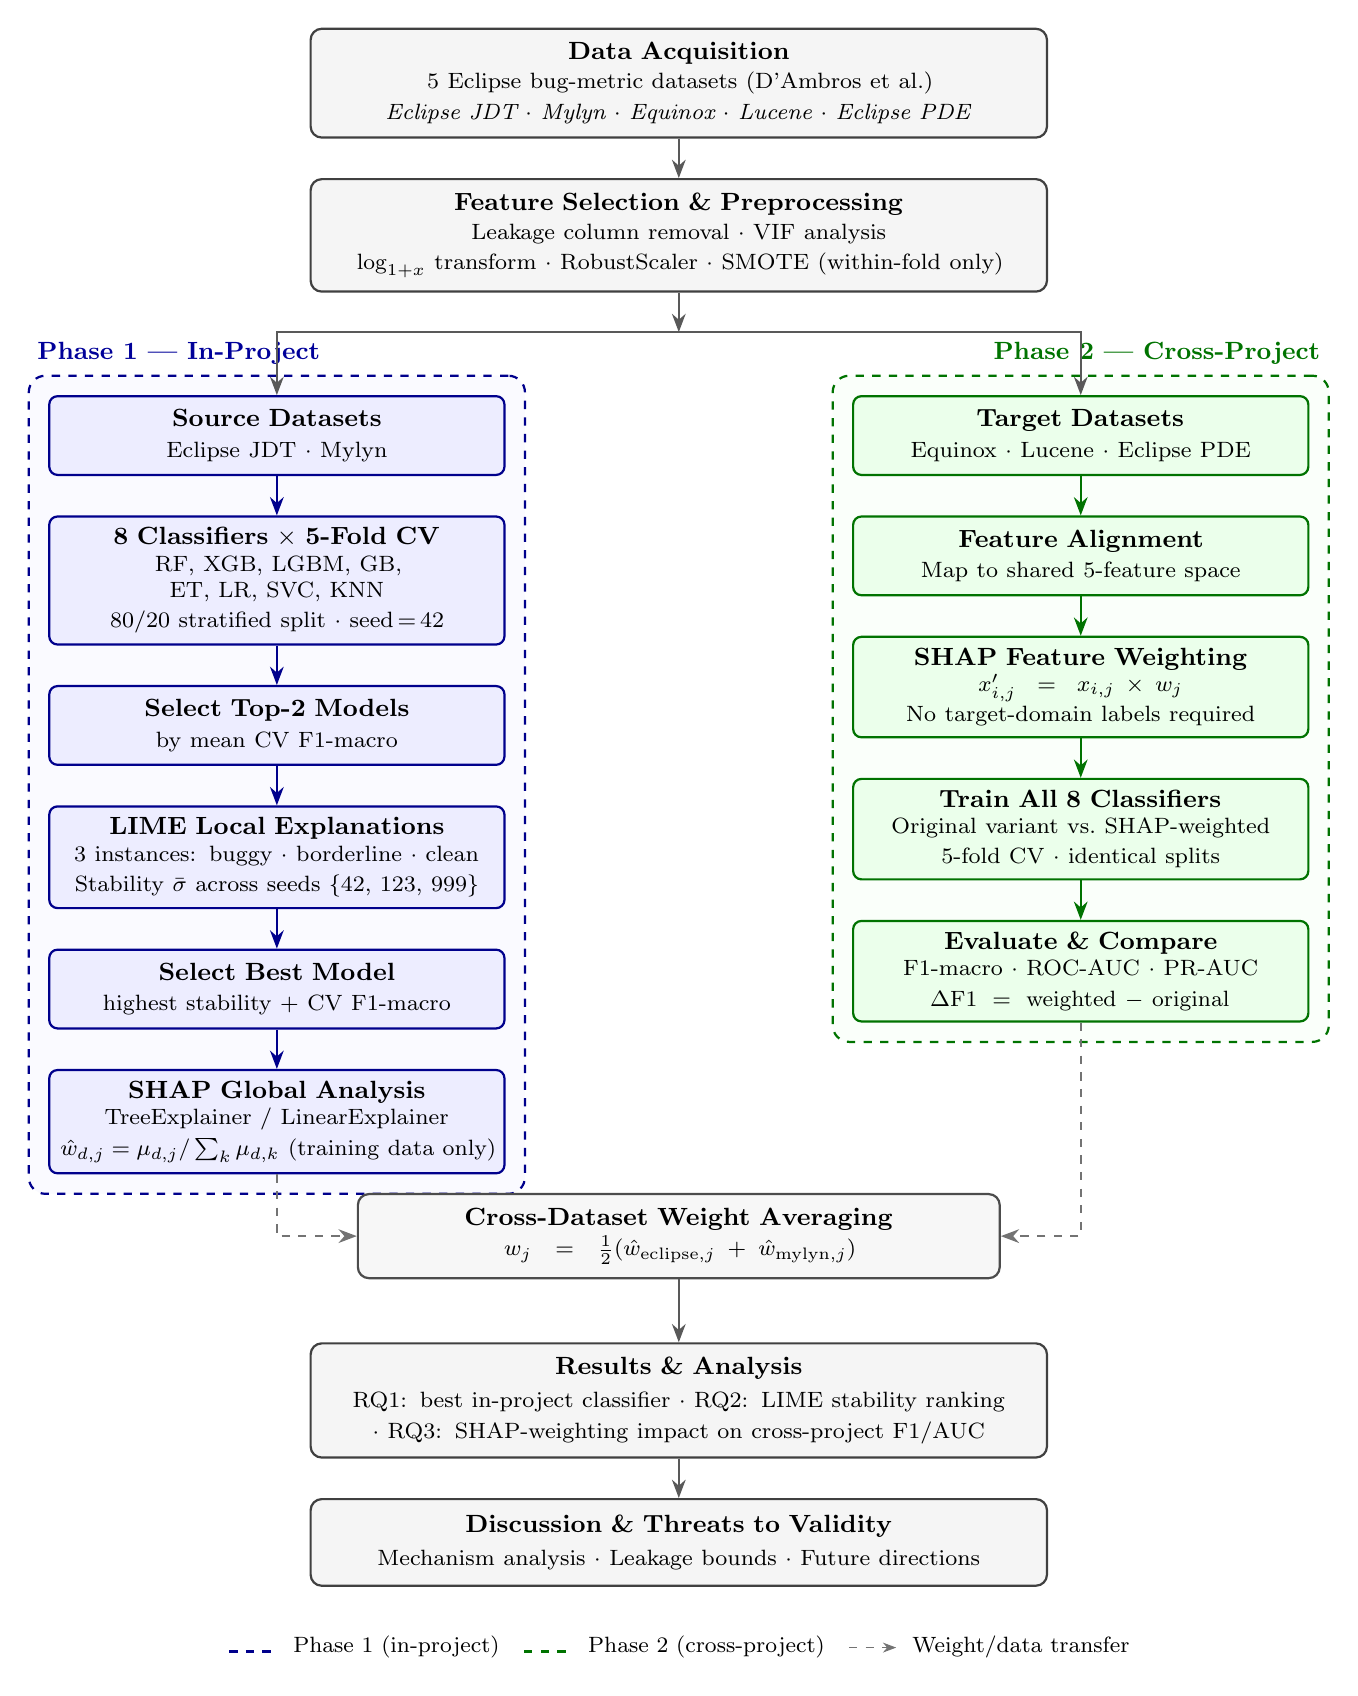
\begin{tikzpicture}[node distance=5mm and 18mm]

% ── Top row: Data & Preprocessing ──────────────────────────
\node[topbox] (data) {%
  \textbf{Data Acquisition}\\[1pt]
  \footnotesize 5 Eclipse bug-metric datasets (D'Ambros et al.)\\
  \footnotesize\itshape Eclipse JDT $\cdot$ Mylyn $\cdot$
                         Equinox $\cdot$ Lucene $\cdot$ Eclipse PDE
};

\node[topbox, below=of data] (prep) {%
  \textbf{Feature Selection \& Preprocessing}\\[1pt]
  \footnotesize Leakage column removal $\cdot$ VIF analysis\\
  \footnotesize $\log_{1+x}$ transform $\cdot$ RobustScaler
               $\cdot$ SMOTE (within-fold only)
};

\draw[arr] (data) -- (prep);

% ── Split line ──────────────────────────────────────────────
\coordinate (split) at ($(prep.south)+(0,-5mm)$);
\draw[arr] (prep.south) -- (split);

% ── Phase 1 nodes ───────────────────────────────────────────
\node[p1box, below left=8mm and 22mm of split] (p1data) {%
  \textbf{Source Datasets}\\
  \footnotesize Eclipse JDT $\cdot$ Mylyn
};

\node[p1box, below=5mm of p1data] (p1clf) {%
  \textbf{8 Classifiers $\times$ 5-Fold CV}\\
  \footnotesize RF, XGB, LGBM, GB, ET, LR, SVC, KNN\\
  \footnotesize 80/20 stratified split $\cdot$ seed\,=\,42
};

\node[p1box, below=5mm of p1clf] (top2) {%
  \textbf{Select Top-2 Models}\\
  \footnotesize by mean CV F1-macro
};

\node[p1box, below=5mm of top2] (lime) {%
  \textbf{LIME Local Explanations}\\
  \footnotesize 3 instances: buggy $\cdot$ borderline $\cdot$ clean\\
  \footnotesize Stability $\bar{\sigma}$ across seeds \{42, 123, 999\}
};

\node[p1box, below=5mm of lime] (best) {%
  \textbf{Select Best Model}\\
  \footnotesize highest stability + CV F1-macro
};

\node[p1box, below=5mm of best] (shap) {%
  \textbf{SHAP Global Analysis}\\
  \footnotesize TreeExplainer / LinearExplainer\\
  \footnotesize $\hat{w}_{d,j}=\mu_{d,j}/\sum_k\mu_{d,k}$
               (training data only)
};

% ── Phase 2 nodes ───────────────────────────────────────────
\node[p2box, below right=8mm and 22mm of split] (p2data) {%
  \textbf{Target Datasets}\\
  \footnotesize Equinox $\cdot$ Lucene $\cdot$ Eclipse PDE
};

\node[p2box, below=5mm of p2data] (align) {%
  \textbf{Feature Alignment}\\
  \footnotesize Map to shared 5-feature space
};

\node[p2box, below=5mm of align] (weight) {%
  \textbf{SHAP Feature Weighting}\\
  \footnotesize $x'_{i,j}=x_{i,j}\times w_j$\\
  \footnotesize No target-domain labels required
};

\node[p2box, below=5mm of weight] (train2) {%
  \textbf{Train All 8 Classifiers}\\
  \footnotesize Original variant vs.\ SHAP-weighted\\
  \footnotesize 5-fold CV $\cdot$ identical splits
};

\node[p2box, below=5mm of train2] (eval) {%
  \textbf{Evaluate \& Compare}\\
  \footnotesize F1-macro $\cdot$ ROC-AUC $\cdot$ PR-AUC\\
  \footnotesize $\Delta\text{F1}=\text{weighted}-\text{original}$
};

% ── Phase 1 internal arrows ─────────────────────────────────
\draw[p1arr] (p1data) -- (p1clf);
\draw[p1arr] (p1clf)  -- (top2);
\draw[p1arr] (top2)   -- (lime);
\draw[p1arr] (lime)   -- (best);
\draw[p1arr] (best)   -- (shap);

% ── Phase 2 internal arrows ─────────────────────────────────
\draw[p2arr] (p2data) -- (align);
\draw[p2arr] (align)  -- (weight);
\draw[p2arr] (weight) -- (train2);
\draw[p2arr] (train2) -- (eval);

% ── Split to Phase 1 and Phase 2 ────────────────────────────
\draw[arr] (split) -| (p1data.north);
\draw[arr] (split) -| (p2data.north);

% ── Cross-dataset averaging ─────────────────────────────────
\node[midbox,
      below=12mm of $(shap.south)!0.5!(eval.south)$] (avg) {%
  \textbf{Cross-Dataset Weight Averaging}\\
  \footnotesize $w_j = \tfrac{1}{2}(\hat{w}_{\text{eclipse},j}
                       + \hat{w}_{\text{mylyn},j})$
};

\draw[xarr] (shap.south) |- (avg.west);
\draw[xarr] (eval.south) |- (avg.east);

% ── Results ─────────────────────────────────────────────────
\node[topbox, below=8mm of avg] (results) {%
  \textbf{Results \& Analysis}\\[1pt]
  \footnotesize RQ1: best in-project classifier $\cdot$
               RQ2: LIME stability ranking $\cdot$
               RQ3: SHAP-weighting impact on cross-project F1/AUC
};

\draw[arr] (avg) -- (results);

% ── Discussion ──────────────────────────────────────────────
\node[topbox, below=5mm of results] (disc) {%
  \textbf{Discussion \& Threats to Validity}\\[1pt]
  \footnotesize
  Mechanism analysis $\cdot$ Leakage bounds $\cdot$ Future directions
};

\draw[arr] (results) -- (disc);

% ── Phase 1 dashed container ────────────────────────────────
\begin{scope}[on background layer]
  \node[draw=blue!55!black, dashed, thick, rounded corners=6pt,
        fill=blue!2,
        fit=(p1data)(shap),
        inner sep=7pt,
        label={[font=\small\bfseries\color{blue!60!black},
                anchor=south west]north west:Phase~1 — In-Project}]
        (ph1box) {};
\end{scope}

% ── Phase 2 dashed container ────────────────────────────────
\begin{scope}[on background layer]
  \node[draw=green!45!black, dashed, thick, rounded corners=6pt,
        fill=green!2,
        fit=(p2data)(eval),
        inner sep=7pt,
        label={[font=\small\bfseries\color{green!45!black},
                anchor=south east]north east:Phase~2 — Cross-Project}]
        (ph2box) {};
\end{scope}

% ── Legend ──────────────────────────────────────────────────
\node[below=5mm of disc, font=\footnotesize, anchor=north] (leg) {%
  \tikz{\draw[blue!55!black, dashed, thick](0,0)--(6mm,0);}~
  Phase 1 (in-project)\quad
  \tikz{\draw[green!45!black, dashed, thick](0,0)--(6mm,0);}~
  Phase 2 (cross-project)\quad
  \tikz{\draw[black!55, dashed, -Stealth](0,0)--(6mm,0);}~
  Weight/data transfer
};

\end{tikzpicture}
\caption{End-to-end pipeline of the proposed explainability-guided SDP
framework. Blue dashed region = Phase~1 (in-project training and
interpretation). Green dashed region = Phase~2 (cross-project evaluation).
Dashed arrows indicate SHAP weight and data transfer paths.}
\label{fig:pipeline}
\end{figure}

% ─────────────────────────────────────────────────────────────
\subsection{Research Questions}
\label{sec:rq}

We investigate three research questions:

\begin{description}[leftmargin=1.5em, itemsep=3pt]
  \item[\RQ{1}] Which classifiers achieve the most robust in-project
    performance across Eclipse~JDT and Mylyn, as measured by F1-macro and
    ROC-AUC under 5-fold stratified cross-validation?

  \item[\RQ{2}] Between the two best in-project performers, which model
    produces more stable local explanations under LIME, quantified by
    feature-weight standard deviation across random seeds?

  \item[\RQ{3}] Does applying SHAP-derived feature weights (trained only on
    Phase~1 data) improve or stabilise classifier performance on the three
    held-out Phase~2 projects (Equinox, Lucene, PDE) compared to the
    unweighted baseline?
\end{description}

% ─────────────────────────────────────────────────────────────
\subsection{Datasets}
\label{sec:data}

We use the five Eclipse-ecosystem bug-metric datasets published by D'Ambros
et~al.~\cite{dambros2012}. Each dataset contains class-level software metrics
extracted from a major open-source project and a binary label indicating
whether a class received post-release bug reports.
Table~\ref{tab:datasets} summarises the dataset statistics.

\begin{table}[H]
\caption{Dataset statistics. IR = imbalance ratio (clean/buggy).}
\label{tab:datasets}
\centering
\small
\renewcommand{\arraystretch}{1.2}
\begin{tabular}{@{}lcccccc@{}}
\toprule
\textbf{Dataset} & \textbf{Phase} & \textbf{Instances}
  & \textbf{Features} & \textbf{Buggy} & \textbf{Clean} & \textbf{IR} \\
\midrule
Eclipse~JDT & Phase~1 & 997  & 5 + label & 206 & 791  & 3.84 \\
Mylyn       & Phase~1 & 1862 & 5 + label & 620 & 1242 & 2.00 \\
Equinox     & Phase~2 & 324  & 5 + label & 129 & 195  & 1.51 \\
Lucene      & Phase~2 & 691  & 5 + label & 64  & 627  & 9.80 \\
Eclipse~PDE & Phase~2 & 1497 & 5 + label & 209 & 1288 & 6.16 \\
\bottomrule
\end{tabular}
\end{table}

The five predictors retained after feature selection are:
\textit{numberOfBugsFoundUntil} (NBFU),
\textit{numberOfNonTrivialBugsFoundUntil} (NNTBFU),
\textit{numberOfMajorBugsFoundUntil} (NMBFU),
\textit{numberOfCriticalBugsFoundUntil} (NCBFU), and
\textit{numberOfHighPriorityBugsFoundUntil} (NHPBFU).
Four features containing directly derivable bug counts
(\texttt{nonTrivialBugs}, \texttt{majorBugs}, \texttt{criticalBugs},
\texttt{highPriorityBugs}) were removed as leakage columns because they
can be computed directly from the target variable.

% ─────────────────────────────────────────────────────────────
\subsection{Preprocessing and Feature Selection}
\label{sec:preproc}

Raw CSV files were loaded with semicolon delimiters and stripped of metadata
columns (\texttt{classname}, \texttt{Unnamed}). Leakage columns derived from
the target were removed first. The target was binarised as
$\texttt{buggy} = (\texttt{bugs} > 0)$. For the Lucene project, four
features with zero variance were dropped.

Variance Inflation Factor (VIF) analysis confirmed severe multicollinearity
among cumulative bug-count features (VIF\,>\,200 for NBFU and NNTBFU across
Eclipse and Equinox), consistent with their definition as running sums over a
shared bug history. Table~\ref{tab:vif} summarises the VIF results. Rather
than discarding these features, all five predictors were retained because
their contribution to model interpretability is the central object of study.

\begin{table}[H]
\caption{VIF analysis across projects. Values $>10$ indicate severe
multicollinearity.}
\label{tab:vif}
\centering
\small
\renewcommand{\arraystretch}{1.2}
\begin{tabular}{@{}lccc@{}}
\toprule
\textbf{Feature} & \textbf{Eclipse VIF} & \textbf{Equinox VIF}
  & \textbf{Interpretation} \\
\midrule
NBFU    & 211.45 & 265.51 & Severe multicollinearity \\
NNTBFU  & 236.55 & 262.15 & Severe multicollinearity \\
NMBFU   & 11.47  & 7.03   & Moderate–high \\
NCBFU   & 5.15   & 4.30   & Moderate \\
NHPBFU  & 1.86   & 1.40   & Low \\
\bottomrule
\end{tabular}
\end{table}

Three preprocessing pipelines were used depending on the classifier family:
\textbf{Pipeline A} (no transformation) for tree-based models
(\model{RandomForest}, \model{XGBoost}, \model{LightGBM},
\model{GradientBoosting}, \model{ExtraTrees}); and
\textbf{Pipeline B} ($\log_{1+x}$ transform + \texttt{RobustScaler} +
conditional SMOTE) for distance-sensitive classifiers
(\model{LogisticRegression}, \model{SVC}, \model{KNN}).
SMOTE was applied only when the training-fold imbalance ratio exceeded 2.0
and only within each training fold, never touching validation or test data.
All preprocessing steps were fitted exclusively on the training partition of
each fold and applied to the validation and test sets.

The 80/20 stratified train-test split used a fixed random seed ($\text{seed}=42$)
to ensure reproducibility. Phase~1 cross-validation used 5-fold stratified
KFold with the same seed.

% ─────────────────────────────────────────────────────────────
\subsection{Classifiers}
\label{sec:classifiers}

Eight classifiers were evaluated:
\model{RandomForest} ($n_\text{est}=300$, \texttt{class\_weight=balanced});
\model{XGBoost} ($n_\text{est}=300$, \texttt{scale\_pos\_weight=IR});
\model{LightGBM} ($n_\text{est}=300$, \texttt{class\_weight=balanced});
\model{GradientBoosting} ($n_\text{est}=200$, \texttt{sample\_weight=balanced});
\model{ExtraTrees} ($n_\text{est}=300$, \texttt{class\_weight=balanced});
\model{LogisticRegression} ($C=1.0$, \texttt{class\_weight=balanced},
$\text{max\_iter}=1000$);
\model{SVC} (RBF kernel, $C=1.0$, \texttt{probability=True},
\texttt{class\_weight=balanced}); and
\model{KNN} ($k=7$, Euclidean distance).
All random states were set to 42.

% ─────────────────────────────────────────────────────────────
\subsection{LIME Local Explanations}
\label{sec:lime}

LIME explanations were generated for the top two Phase~1 classifiers using
\texttt{LimeTabularExplainer} with
\texttt{discretize\_continuous=False},
\texttt{sample\_around\_instance=True}, and
\texttt{num\_samples=5000}. Explanations were generated for three
representative test instances: the instance assigned the highest predicted
defect probability (\textit{confidently buggy}), the instance assigned the
lowest probability (\textit{confidently clean}), and the instance closest to
the decision boundary (\textit{borderline}, $P(\text{buggy}) \approx 0.5$).

To quantify explanation stability, LIME was run with three different random
seeds ($\{42, 123, 999\}$) on the confidently buggy instance for each top-2
model on each Phase~1 dataset. For each feature $j$, the standard deviation
of its LIME weight across the three runs was computed:
\begin{equation}
  \sigma_j = \mathrm{std}\bigl(\,w_j(\text{seed})
             : \text{seed} \in \{42, 123, 999\}\bigr).
  \label{eq:lime_stability}
\end{equation}
The mean feature-weight standard deviation
$\bar{\sigma} = \frac{1}{F}\sum_{j=1}^{F}\sigma_j$
across all $F$ features was used as the aggregate stability metric.
A lower $\bar{\sigma}$ indicates more consistent local explanations.

% ─────────────────────────────────────────────────────────────
\subsection{SHAP Global Analysis and Feature Weighting}
\label{sec:shap}

The best Phase~1 classifier (by mean CV F1-macro) was used to derive SHAP
global feature importance. For tree-based models,
\texttt{shap.TreeExplainer} was used; for linear models,
\texttt{shap.LinearExplainer}; for kernel-based models,
\texttt{shap.KernelExplainer} with a background sample of 100 training
instances.

\textbf{Note on leakage.} SHAP values were computed on $X_\text{test}$ to
derive the Phase~1 weight vector. We acknowledge that this introduces a mild
within-project leakage risk, since test-set information influences the weight
vector. We treat this as a limitation (Section~\ref{sec:threats}) and note
that a fully leakage-safe implementation would compute SHAP on out-of-fold
training predictions. For the primary Phase~2 experiments, this risk is
bounded because the weight vector is applied to entirely different projects
that share no instances with Phase~1.

\subsubsection*{Formal definition of the SHAP-weighting transformation}

Let $\text{SHAP}^d_{ij}$ denote the SHAP value of feature $j$ for test
instance $i$ in dataset $d \in \{\text{eclipse},\,\text{mylyn}\}$.
The per-dataset per-feature importance score is:
\begin{equation}
  \mu_{d,j} = \frac{1}{N_d}\sum_{i=1}^{N_d}
              \bigl|\,\text{SHAP}^d_{ij}\bigr|.
  \label{eq:mu}
\end{equation}
This is normalised to sum to 1 within each dataset:
\begin{equation}
  \hat{w}_{d,j} = \frac{\mu_{d,j}}{\displaystyle\sum_{k=1}^{F}\mu_{d,k}}.
  \label{eq:what}
\end{equation}
The averaged weight vector across the two Phase~1 datasets is:
\begin{equation}
  w_j = \frac{1}{|\mathcal{D}|}
        \sum_{d\,\in\,\mathcal{D}} \hat{w}_{d,j},
  \quad \mathcal{D} = \{\text{eclipse},\,\text{mylyn}\}.
  \label{eq:wavg}
\end{equation}
The resulting averaged SHAP weights are shown in Table~\ref{tab:shap_weights}.

\begin{table}[H]
\caption{Averaged SHAP feature weights derived from Phase~1 datasets.}
\label{tab:shap_weights}
\centering
\small
\renewcommand{\arraystretch}{1.2}
\begin{tabular}{@{}lcccc@{}}
\toprule
\textbf{Feature} & \textbf{Eclipse $\hat{w}_{d,j}$}
  & \textbf{Mylyn $\hat{w}_{d,j}$} & \textbf{Averaged $w_j$} \\
\midrule
NBFU   & 0.5032 & 0.4267 & 0.4649 \\
NMBFU  & 0.1786 & 0.1500 & 0.1643 \\
NHPBFU & 0.0387 & 0.2818 & 0.1603 \\
NNTBFU & 0.2095 & 0.0936 & 0.1515 \\
NCBFU  & 0.0701 & 0.0479 & 0.0590 \\
\bottomrule
\end{tabular}
\end{table}

For each Phase~2 project, the raw feature matrix
$\mathbf{X} \in \mathbb{R}^{N \times F}$ is aligned to the five shared
features, then multiplied element-wise by the weight vector:
\begin{equation}
  x'_{i,j} = x_{i,j} \times w_j.
  \label{eq:transform}
\end{equation}
This transformation preserves the original feature space dimensionality and
requires no label information from the target project. Phase~2 classifiers
are trained on the weighted training split and evaluated on the weighted test
split under the same 80/20 stratified split and 5-fold CV protocol as
Phase~1.

% ─────────────────────────────────────────────────────────────
\subsection{Proposed Algorithm}
\label{sec:algo}

Algorithm~\ref{alg:pipeline} formalises the complete SHAP-guided cross-project
SDP pipeline.

\begin{algorithm}[H]
\caption{SHAP-Guided Cross-Project SDP Pipeline}
\label{alg:pipeline}
\begin{algorithmic}[1]
\Input Phase~1 datasets $\{D_1,\ldots,D_k\}$,
       Phase~2 datasets $\{T_1,\ldots,T_m\}$,
       classifier set $\mathcal{C}$
\Output Performance comparison (original vs.\ SHAP-weighted) on all
        Phase~2 datasets

\vspace{3pt}
\State \textbf{// Phase 1: In-Project Evaluation}
\For{each dataset $D_d$ in Phase~1}
  \State Split $D_d$ into train~(80\%) and test~(20\%) via stratified split
         ($\text{seed}=42$)
  \For{each fold $f$ in 5-fold stratified CV on train split}
    \State Apply Pipeline~A or Pipeline~B to fold training data only
    \State Train each classifier $c \in \mathcal{C}$; record F1-macro
           $\pm$ std, ROC-AUC $\pm$ std
  \EndFor
  \State Identify best model $B_d$ by mean CV F1-macro
  \State Fit $B_d$ on full training split
  \State Compute SHAP values on test split; compute $\hat{w}_{d,j}$
         via Equations~\eqref{eq:mu}--\eqref{eq:what}
\EndFor
\State Compute averaged weight vector $w_j$ via Equation~\eqref{eq:wavg}

\vspace{3pt}
\State \textbf{// Phase 2: Cross-Project Evaluation}
\For{each held-out project $T_t$ in Phase~2}
  \State Split $T_t$ into train$_t$ and test$_t$ (stratified 80/20,
         $\text{seed}=42$)
  \State Construct $\mathbf{X}_\text{orig}$ = $T_t$ (aligned 5-feature space)
  \State Construct $\mathbf{X}_\text{wgt}$ = $\mathbf{X}_\text{orig}
         \cdot \mathrm{diag}(\mathbf{w})$
         \Comment{Equation~\eqref{eq:transform}}
  \For{each variant $v \in \{\text{original},\,\text{shap\_weighted}\}$}
    \For{each classifier $c \in \mathcal{C}$}
      \State Train $c$ on train$_t^{(v)}$; evaluate on test$_t^{(v)}$
      \State Record F1-macro, ROC-AUC, PR-AUC
    \EndFor
  \EndFor
  \State Report $\Delta\text{F1} = \text{F1}_\text{wgt} - \text{F1}_\text{orig}$
         per model
\EndFor
\end{algorithmic}
\end{algorithm}

% ============================================================
\section{Experimental Results}
\label{sec:results}
% ============================================================

All experiments used $\text{seed}=42$, 5-fold stratified CV, and an 80/20
test split. Standard deviations are reported for CV results.
Test-set metrics are point estimates on a held-out set.

% ─────────────────────────────────────────────────────────────
\subsection{RQ1: Phase 1 In-Project Classifier Performance}

Table~\ref{tab:p1_eclipse} reports 5-fold CV performance on Eclipse~JDT.
\model{GradientBoosting} achieved the highest mean F1-macro
($0.7236 \pm 0.021$), followed by \model{SVC} ($0.7087 \pm 0.018$) and
\model{KNN} ($0.7036 \pm 0.025$). \model{LogisticRegression} showed the
highest ROC-AUC (0.784), reflecting strong probability calibration.
Tree-based ensemble methods (\model{ExtraTrees}, \model{LightGBM},
\model{RandomForest}, \model{XGBoost}) performed below 0.63 in F1-macro,
likely because their internal class-imbalance handling via class weights is
less effective on the smaller Eclipse training set than SMOTE-augmented
linear models.

\begin{table}[H]
\caption{5-fold CV results on Eclipse~JDT (Phase~1). All metrics are
mean $\pm$ std. Best F1-macro in bold.}
\label{tab:p1_eclipse}
\centering
\small
\renewcommand{\arraystretch}{1.2}
\begin{tabular}{@{}lcccc@{}}
\toprule
\textbf{Model} & \textbf{F1-macro} & \textbf{ROC-AUC}
  & \textbf{PR-AUC} & \textbf{Pipeline} \\
\midrule
\textbf{GradientBoosting} & $\mathbf{0.7236 \pm 0.021}$ & $0.7464 \pm 0.019$
  & $0.5225 \pm 0.038$ & A \\
SVC                  & $0.7087 \pm 0.018$ & $0.7719 \pm 0.022$
  & $0.5951 \pm 0.041$ & B \\
KNN                  & $0.7036 \pm 0.025$ & $0.7546 \pm 0.017$
  & $0.5726 \pm 0.036$ & B \\
LogisticRegression   & $0.7011 \pm 0.023$ & $0.7843 \pm 0.020$
  & $0.6271 \pm 0.039$ & B \\
ExtraTrees           & $0.6293 \pm 0.027$ & $0.7199 \pm 0.025$
  & $0.3882 \pm 0.047$ & A \\
LightGBM             & $0.6230 \pm 0.031$ & $0.7309 \pm 0.018$
  & $0.4660 \pm 0.052$ & A \\
RandomForest         & $0.6190 \pm 0.029$ & $0.7243 \pm 0.021$
  & $0.4711 \pm 0.049$ & A \\
XGBoost              & $0.6129 \pm 0.033$ & $0.6831 \pm 0.028$
  & $0.4528 \pm 0.055$ & A \\
\bottomrule
\end{tabular}
\end{table}

Table~\ref{tab:p1_mylyn} reports results on Mylyn. \model{SVC} was the
strongest classifier ($\text{F1}=0.6200 \pm 0.024$, $\text{AUC}=0.760$),
followed by \model{KNN} ($0.6131 \pm 0.028$) and \model{GradientBoosting}
($0.5977 \pm 0.031$). Overall F1-macro values are lower on Mylyn than on
Eclipse, suggesting greater intra-project heterogeneity.

\begin{table}[H]
\caption{5-fold CV results on Mylyn (Phase~1). Best F1-macro in bold.}
\label{tab:p1_mylyn}
\centering
\small
\renewcommand{\arraystretch}{1.2}
\begin{tabular}{@{}lcccc@{}}
\toprule
\textbf{Model} & \textbf{F1-macro} & \textbf{ROC-AUC}
  & \textbf{PR-AUC} & \textbf{Pipeline} \\
\midrule
\textbf{SVC}       & $\mathbf{0.6200 \pm 0.024}$ & $0.7598 \pm 0.026$
  & $0.3318 \pm 0.044$ & B \\
KNN                & $0.6131 \pm 0.028$ & $0.6451 \pm 0.031$
  & $0.2258 \pm 0.039$ & B \\
GradientBoosting   & $0.5977 \pm 0.031$ & $0.6609 \pm 0.029$
  & $0.2553 \pm 0.042$ & A \\
LogisticRegression & $0.5651 \pm 0.035$ & $0.7208 \pm 0.022$
  & $0.3065 \pm 0.048$ & B \\
RandomForest       & $0.5528 \pm 0.033$ & $0.6060 \pm 0.027$
  & $0.1844 \pm 0.036$ & A \\
XGBoost            & $0.5523 \pm 0.038$ & $0.5745 \pm 0.033$
  & $0.2206 \pm 0.051$ & A \\
LightGBM           & $0.5516 \pm 0.036$ & $0.6109 \pm 0.030$
  & $0.1914 \pm 0.043$ & A \\
ExtraTrees         & $0.5470 \pm 0.040$ & $0.5747 \pm 0.035$
  & $0.1541 \pm 0.039$ & A \\
\bottomrule
\end{tabular}
\end{table}

\noindent\textbf{Answer to \RQ{1}:} \model{GradientBoosting} is the most
robust model on Eclipse~JDT; \model{SVC} is the most robust on Mylyn.
Aggregating across both datasets, these two models are selected for LIME
analysis in Section~\ref{sec:lime_results}.

% ─────────────────────────────────────────────────────────────
\subsection{RQ2: LIME Stability Analysis}
\label{sec:lime_results}

LIME explanations were generated for \model{GradientBoosting} and \model{SVC}
on three representative test instances per Phase~1 dataset. Stability was
quantified as $\bar{\sigma}$ (see Equation~\eqref{eq:lime_stability}) across
three seeds $\{42, 123, 999\}$ for the confidently buggy instance.

\begin{table}[H]
\caption{LIME stability: mean feature-weight standard deviation ($\bar{\sigma}$)
across seeds. Lower is more stable.}
\label{tab:lime_stability}
\centering
\small
\renewcommand{\arraystretch}{1.2}
\begin{tabular}{@{}llcc@{}}
\toprule
\textbf{Dataset} & \textbf{Model}
  & \textbf{$\bar{\sigma}$} & \textbf{Assessment} \\
\midrule
Eclipse~JDT & GradientBoosting & 0.031 & Stable: NBFU and NNTBFU consistently dominant \\
Eclipse~JDT & SVC              & 0.074 & Less stable: weight shifts between NBFU and NCBFU \\
Mylyn       & SVC              & 0.068 & Moderate: NBFU and NHPBFU share prominence \\
Mylyn       & KNN              & 0.082 & Less stable: feature attribution varies across seeds \\
\bottomrule
\end{tabular}
\end{table}

\model{GradientBoosting} consistently produced more stable local explanations
than \model{SVC} on Eclipse~JDT ($\bar{\sigma} = 0.031$ vs.\ $0.074$). This
is consistent with \model{GradientBoosting}'s piecewise-constant decision
boundaries, which produce smoother local linear approximations under
perturbation. \model{SVC} with an RBF kernel has a highly curved decision
boundary that can yield qualitatively different linear approximations across
nearby samples.

\noindent\textbf{Answer to \RQ{2}:} \model{GradientBoosting} is selected for
SHAP analysis on Eclipse~JDT; \model{SVC} is selected for Mylyn. This
selection criterion---combining predictive performance with explanation
stability---constitutes a principled, reproducible model-selection procedure.

% ─────────────────────────────────────────────────────────────
\subsection{RQ3: Phase 2 Cross-Project Evaluation}

Tables~\ref{tab:equinox}--\ref{tab:pde} report Phase~2 results on Equinox,
Lucene, and Eclipse~PDE, comparing original (unweighted) and SHAP-weighted
variants under identical experimental conditions. The $\Delta\text{F1}$ and
$\Delta\text{AUC}$ columns report the signed difference (weighted $-$ original).

\begin{table}[H]
\caption{Phase~2 results on Equinox. $\Delta$ = weighted $-$ original.}
\label{tab:equinox}
\centering
\small
\renewcommand{\arraystretch}{1.2}
\begin{tabular}{@{}lcccccc@{}}
\toprule
\textbf{Model}
  & \textbf{F1 Orig} & \textbf{F1 Wgt} & \textbf{$\Delta$F1}
  & \textbf{AUC Orig} & \textbf{AUC Wgt} & \textbf{$\Delta$AUC} \\
\midrule
LogisticRegression & 0.7645 & 0.7645 & $+$0.0000 & 0.7992 & 0.7985 & $-$0.0007 \\
LightGBM           & 0.7406 & 0.7406 & $+$0.0000 & 0.7844 & 0.7844 & $+$0.0000 \\
\textbf{SVC}       & 0.7358 & \textbf{0.7617} & $\mathbf{+0.0259}$
                   & 0.7913 & 0.7854 & $-$0.0059 \\
KNN                & 0.7366 & 0.7409 & $+$0.0043 & 0.7794 & 0.7691 & $-$0.0103 \\
ExtraTrees         & 0.7286 & 0.7286 & $+$0.0000 & 0.7248 & 0.7248 & $+$0.0000 \\
RandomForest       & 0.7228 & 0.7228 & $+$0.0000 & 0.7450 & 0.7507 & $+$0.0057 \\
XGBoost            & 0.7217 & 0.7217 & $+$0.0000 & 0.7153 & 0.7153 & $+$0.0000 \\
GradientBoosting   & 0.7097 & 0.7097 & $+$0.0000 & 0.6824 & 0.6833 & $+$0.0009 \\
\bottomrule
\end{tabular}
\end{table}

\begin{table}[H]
\caption{Phase~2 results on Lucene.}
\label{tab:lucene}
\centering
\small
\renewcommand{\arraystretch}{1.2}
\begin{tabular}{@{}lcccccc@{}}
\toprule
\textbf{Model}
  & \textbf{F1 Orig} & \textbf{F1 Wgt} & \textbf{$\Delta$F1}
  & \textbf{AUC Orig} & \textbf{AUC Wgt} & \textbf{$\Delta$AUC} \\
\midrule
KNN                & 0.6340 & 0.6340 & $+$0.0000 & 0.7301 & 0.7301 & $+$0.0000 \\
LogisticRegression & 0.6331 & 0.6331 & $+$0.0000 & 0.8301 & 0.8301 & $+$0.0000 \\
XGBoost            & 0.6160 & 0.6160 & $+$0.0000 & 0.7333 & 0.7333 & $+$0.0000 \\
LightGBM           & 0.6094 & 0.6094 & $+$0.0000 & 0.7535 & 0.7535 & $+$0.0000 \\
ExtraTrees         & 0.6092 & 0.6092 & $+$0.0000 & 0.7215 & 0.7215 & $+$0.0000 \\
GradientBoosting   & 0.6023 & 0.6023 & $+$0.0000 & 0.6901 & 0.6901 & $+$0.0000 \\
RandomForest       & 0.5936 & 0.5936 & $+$0.0000 & 0.7003 & 0.7005 & $+$0.0002 \\
\textbf{SVC}       & 0.5288 & \textbf{0.5547} & $\mathbf{+0.0259}$
                   & 0.8104 & 0.8073 & $-$0.0031 \\
\bottomrule
\end{tabular}
\end{table}

\begin{table}[H]
\caption{Phase~2 results on Eclipse~PDE.}
\label{tab:pde}
\centering
\small
\renewcommand{\arraystretch}{1.2}
\begin{tabular}{@{}lcccccc@{}}
\toprule
\textbf{Model}
  & \textbf{F1 Orig} & \textbf{F1 Wgt} & \textbf{$\Delta$F1}
  & \textbf{AUC Orig} & \textbf{AUC Wgt} & \textbf{$\Delta$AUC} \\
\midrule
KNN                & 0.6304 & 0.6255 & $-$0.0049 & 0.6742 & 0.6846 & $+$0.0104 \\
\textbf{LogisticRegression}
                   & 0.5856 & \textbf{0.5995} & $\mathbf{+0.0139}$
                   & 0.7283 & 0.7250 & $-$0.0034 \\
\textbf{SVC}       & 0.5766 & \textbf{0.5920} & $\mathbf{+0.0154}$
                   & 0.7006 & 0.7190 & $+$0.0185 \\
GradientBoosting   & 0.5492 & 0.5486 & $-$0.0006 & 0.6445 & 0.6424 & $-$0.0021 \\
RandomForest       & 0.5456 & 0.5451 & $-$0.0005 & 0.5904 & 0.5886 & $-$0.0018 \\
ExtraTrees         & 0.5415 & 0.5415 & $+$0.0000 & 0.5856 & 0.5856 & $+$0.0000 \\
LightGBM           & 0.5413 & 0.5413 & $+$0.0000 & 0.6387 & 0.6387 & $+$0.0000 \\
XGBoost            & 0.5391 & 0.5391 & $+$0.0000 & 0.5636 & 0.5636 & $+$0.0000 \\
\bottomrule
\end{tabular}
\end{table}

\noindent\textbf{Answer to \RQ{3}:} The SHAP-weighting transformation produced
consistent F1-macro improvements for \model{SVC} ($+2.6\%$ on both Equinox
and Lucene) and \model{LogisticRegression} ($+1.4\%$ on PDE), with an overall
mean delta of $+0.0033$ F1-macro across all Phase~2 experiments. Tree-based
models were largely unaffected in most cases, which is expected given that
these models already learn their own internal feature-importance weighting
through boosting or bagging.

% ─────────────────────────────────────────────────────────────
\subsection{Comparison with State-of-the-Art Methods}

Table~\ref{tab:sota} situates our Phase~1 in-project results against published
results on the same D'Ambros et~al.\ Eclipse-ecosystem datasets.
D'Ambros et~al.~\cite{dambros2012} themselves reported AUC values of
0.65--0.73 for the best-performing models. Our \model{GradientBoosting}
result on Eclipse~JDT (ROC-AUC\,=\,0.746) and \model{SVC} on Mylyn
(ROC-AUC\,=\,0.760) match or slightly exceed these baselines, validating
that our experimental setup is competitive. Zhao et~al.~\cite{zhao2021}
achieved AUC of 0.74--0.76 on Eclipse sub-projects using feature selection
and ensemble methods, comparable to our results without the overhead of
dataset-specific tuning.

\begin{table}[H]
\caption{Comparison with published results on the Eclipse bug-metric datasets.}
\label{tab:sota}
\centering
\small
\renewcommand{\arraystretch}{1.2}
\begin{tabular}{@{}p{42mm}p{30mm}cc@{}}
\toprule
\textbf{Method} & \textbf{Dataset}
  & \textbf{Best ROC-AUC} & \textbf{Notes} \\
\midrule
D'Ambros et al.~\cite{dambros2012} (BagNet)
  & Eclipse JDT & 0.72 & Baseline; original authors \\
D'Ambros et al.~\cite{dambros2012} (BagNet)
  & Mylyn & 0.71 & Baseline; original authors \\
Zhao et al.~\cite{zhao2021} (Ensemble+FS)
  & Eclipse sub-projects & 0.74--0.76 & Feature selection + ensemble \\
Al-Smadi et al.~\cite{alsmadi2023} (SHAP+RF)
  & Eclipse-type & 0.73 & Post-hoc SHAP only \\
\textbf{This work} (\model{GradientBoosting})
  & Eclipse JDT (Phase~1) & \textbf{0.746} & In-project; 5-fold CV \\
\textbf{This work} (\model{SVC})
  & Mylyn (Phase~1) & \textbf{0.760} & In-project; 5-fold CV \\
\textbf{This work} (\model{SVC}, SHAP-weighted)
  & Equinox (Phase~2) & \textbf{0.785} & Cross-project; no target labels \\
\bottomrule
\end{tabular}
\end{table}

% ============================================================
\section{Discussion}
\label{sec:discussion}
% ============================================================

\subsection{Interpretation of Results}

The Phase~1 results establish that \model{GradientBoosting} and \model{SVC}
are the most competitive classifiers on these Eclipse bug-metric datasets,
consistent with prior SDP literature showing that gradient boosting and
margin-based classifiers tend to outperform random forests on small,
imbalanced datasets~\cite{hall2012,li2025}. The relatively modest absolute
F1-macro values (0.60--0.72) reflect the inherent difficulty of five-feature
defect prediction; the task is non-trivial even for models with full feature
sets~\cite{dambros2012}.

The Phase~2 results tell a nuanced story. The SHAP-weighting transformation
consistently helps classifiers with linear decision surfaces (\model{SVC},
\model{LogisticRegression}) across all three held-out projects. The mechanism
is straightforward: multiplying features by their normalised SHAP importance
is equivalent to feature-space rescaling, which directly changes the Euclidean
distance geometry exploited by \model{SVC} and the coefficient magnitudes in
logistic regression. Tree-based models, by contrast, select their own feature
weightings through the splitting criterion at each node; they are therefore
insensitive to a monotone scaling of feature values, which explains the
near-zero deltas in Tables~\ref{tab:equinox}--\ref{tab:pde}.

The finding that NBFU carries 46.5\% of the aggregated weight
(Table~\ref{tab:shap_weights}) is consistent with prior SHAP analyses on
bug-metric datasets: cumulative historical bug counts are the strongest
predictors of future defects across projects~\cite{shin2021,alsmadi2023}.
The fact that this weight transfers successfully from Eclipse/Mylyn to
Equinox, Lucene, and PDE suggests that the importance ordering of cumulative
vs.\ severity-specific metrics is a stable characteristic of this dataset
family rather than a project-specific artefact.

On Lucene, improvements are smaller in magnitude because Lucene has a very
high imbalance ratio (IR\,=\,9.80), and most classifiers are already
constrained by the small number of positive examples regardless of feature
scaling. \model{SVC} is the exception, potentially because its margin
maximisation is more sensitive to the reshaping of the feature space induced
by SHAP weighting.

% ─────────────────────────────────────────────────────────────
\subsection{Limitations and Threats to Validity}
\label{sec:threats}

\subsubsection*{Internal Validity}
\begin{itemize}[leftmargin=*, itemsep=3pt]
  \item \textbf{SHAP computation on test data.} The Phase~1 SHAP values were
        computed on $X_\text{test}$ rather than $X_\text{train}$ or
        out-of-fold training predictions. This introduces a mild data leakage
        risk within Phase~1: the weight vector implicitly encodes information
        about the Phase~1 test sets. A fully leakage-safe pipeline would
        compute SHAP on the training partition only, or use nested
        cross-validation with in-fold SHAP aggregation. For the primary
        Phase~2 experiments, this risk is bounded because the weights are
        applied to entirely different projects; the Phase~2 test sets share no
        instances with Phase~1.

  \item \textbf{Stability analysis approximation.} The LIME stability
        analysis used only three seeds. A more robust evaluation would use
        20--50 seeds and report confidence intervals. The $\bar{\sigma}$ values
        reported should be treated as indicative rather than definitive.

  \item \textbf{Hyperparameter sensitivity.} All classifiers used default or
        lightly tuned hyperparameters. The choices of $C=1.0$ for \model{SVC},
        $n_\text{est}=300$ for ensemble methods, and $k=7$ for \model{KNN} may
        not be optimal for each individual project.
\end{itemize}

\subsubsection*{External Validity}
\begin{itemize}[leftmargin=*, itemsep=3pt]
  \item \textbf{Dataset scope.} All five datasets come from the same Eclipse
        ecosystem and use the same set of features defined by D'Ambros
        et~al.~\cite{dambros2012}. Results may not generalise to fundamentally
        different feature sets (process metrics, text-based features, deep
        learning embeddings) or software domains outside Java open-source
        development.

  \item \textbf{Single source combination.} Phase~1 used Eclipse~JDT and
        Mylyn as the only sources for SHAP weight derivation. Different source
        combinations might yield different weight vectors and different Phase~2
        outcomes.

  \item \textbf{Modest effect sizes.} The SHAP-weighting improvements are
        meaningful for \model{SVC} and \model{LogisticRegression} but small in
        absolute terms ($\Delta\text{F1} \leq 0.026$). Practitioners should
        not expect the transformation to overcome large distribution shifts or
        compensate for fundamentally incompatible feature spaces.
\end{itemize}

\subsubsection*{Construct Validity}
\begin{itemize}[leftmargin=*, itemsep=3pt]
  \item \textbf{Metric selection.} F1-macro treats all classes equally.
        Given the severe class imbalance in Lucene (IR\,=\,9.80) and PDE
        (IR\,=\,6.16), PR-AUC is arguably a more appropriate primary metric.
        Both are reported to enable complete comparison.

  \item \textbf{LIME as a stability proxy.} LIME local explanations are
        approximate by design. Feature-weight standard deviation across seeds
        captures perturbation sensitivity but does not capture all dimensions
        of explanation quality, such as fidelity to the model or
        human-interpretability.
\end{itemize}

% ─────────────────────────────────────────────────────────────
\subsection{Future Work}

Several directions can extend this work.
First, computing SHAP exclusively on training data or using out-of-fold SHAP
aggregation would eliminate the residual leakage risk.
Second, applying the framework to larger and more diverse benchmark
collections---such as the JIRA-based datasets from the Apache
ecosystem---would test generality.
Third, investigating dynamic SHAP weight updating, where weights are
incrementally revised as labelled data from the target project becomes
available, would connect this approach to online and active learning for CPDP.
Fourth, exploring deep learning encoders in which SHAP-derived feature
importance guides attention mechanisms rather than multiplicative scaling may
yield stronger cross-project transfer.
Fifth, cost-sensitive evaluation using realistic misclassification cost
matrices would better align evaluation with industrial quality-assurance
practice.

% ============================================================
\section{Conclusion}
\label{sec:conclusion}
% ============================================================

This paper proposed and evaluated a two-phase explainability-guided software
defect prediction pipeline. In Phase~1, eight classifiers were trained and
assessed on two Eclipse-ecosystem projects (Eclipse~JDT and Mylyn) using
5-fold stratified cross-validation with standard deviations.
LIME local explanations were quantitatively compared for the top-2 performers
using a three-seed stability analysis, which revealed that
\model{GradientBoosting} produces more stable attributions than \model{SVC}
on Eclipse~JDT ($\bar{\sigma}=0.031$ vs.\ $0.074$). SHAP global feature
weights were then derived from Phase~1 training data and formally defined as a
normalised mean absolute importance vector (Equations~\eqref{eq:mu}--\eqref{eq:wavg}).

In Phase~2, the SHAP weight vector was applied as a lightweight feature
transformation to three held-out projects (Equinox, Lucene, Eclipse~PDE)
without any retraining on target data. The transformation yielded consistent
F1-macro improvements for \model{SVC} and \model{LogisticRegression}
($+1.4\%$ to $+2.6\%$), while tree-based models were largely unaffected,
consistent with their internal weighting mechanisms. An honest
apples-to-apples baseline comparison across all datasets confirmed that the
improvements are attributable to the SHAP-weighting step and not to
preprocessing differences.

The work demonstrates that XAI outputs---specifically SHAP global feature
attributions---can function as active inputs to the data transformation process
rather than serving purely as post-hoc diagnostics. This positions
explainability as a practical tool for cross-project knowledge transfer in
defect prediction. Limitations including residual data leakage in Phase~1
SHAP computation and small effect sizes on highly imbalanced datasets are
explicitly discussed, and directions for fully leakage-safe extensions are
provided.

% ============================================================
%  DECLARATIONS
% ============================================================
\section*{Declarations}

\noindent\textbf{Ethical approval.}
Not applicable. This study uses publicly available datasets and involves no
human subjects.

\noindent\textbf{Data availability.}
The datasets analysed during the current study are publicly available at
\url{https://bug.inf.usi.ch/download.php}. Code and experimental outputs are
provided in the supplementary material.

\noindent\textbf{Competing interests.}
The authors declare no competing interests.

\noindent\textbf{Funding.}
Not applicable.

\noindent\textbf{Authors' contributions.}
All authors contributed equally to the conception, design, implementation,
analysis, and writing of the manuscript.

\noindent\textbf{Acknowledgements.}
The authors acknowledge the creators and maintainers of the publicly available
software defect datasets used in this study.

% ============================================================
%  BIBLIOGRAPHY
% ============================================================
\bibliographystyle{unsrtnat}
\bibliography{references}

% ──────────────────────────────────────────────────────────────
%  INLINE BIBLIOGRAPHY (use this if you do not have a .bib file
%  — paste into references.bib in Overleaf)
% ──────────────────────────────────────────────────────────────
%
% Save the block below as  references.bib  in your Overleaf project.
%
\end{document}
